%Dette er rootfilen til oppgaven: root.tex

%%========================================
\documentclass[12pt]{report}
%\usepackage[norsk]{babel}
\usepackage[utf8]{inputenc}
\usepackage{ramsstyle}
\usepackage{parskip}
\usepackage{graphicx}
\graphicspath{ {pictures/} {pictures/guipictures/} }
\usepackage{array}
\usepackage{cleveref}
\usepackage{pdfpages}
\usepackage{wrapfig}
\usepackage[titletoc,title]{appendix}
\usepackage{paralist}
\usepackage{caption}
\usepackage{subcaption}
\usepackage{listings}
% \usepackage[a-1b]{pdfx}
% \usepackage{hyperref}
\usepackage{comment}


%\addto{\captionsnorsk}{\renewcommand*{\appendixname}{Vedlegg}}

\usepackage[backend=biber]{biblatex}
%\addbibresource{referanser.bib}

% \usepackage{fancyhdr}
% % \usepackage{lipsum} % only for showing some sample text
% \fancyhf{} % clear all header and footers
% \renewcommand{\headrulewidth}{0pt} % remove the header rule
% \rfoot{\thepage}
%%========================================


%%========================================
\begin{document}

\title{Project in sensor systems}
\author{Torbjørn Helmersen}
\date{Autumn 2016\\ Department of technology \\ Norwegian University of Science and Technology\\and\\ Mid Sweden University}


\maketitle

\section*{Preface}

The objective for this project is to build a camera based system for measuring the liquid level in a transparent drain tank, then use the data from the camera to create a feedback for a level control system. This project can further be divided into the following tasks:

\begin{itemize}
    \item Develop a software for detecting and calculating the liquid level in a cylindrical, transparent tank using a RGB camera.
    \item Assemble/prepare a drain tank system ready to measure liquid level.
    \item Write LabView code for Vision Acquisition.
    \item Write PID controller algorithm using LabView to control the pump in the drain tank.
    \item Testing and modulate controller parameters with Ziegler-Nichols tuning method and Integral-Time-Absolute-Error \textbf{(ITAE)} criteria.
    
\end{itemize}

\centerline{Trondheim, 2016} 
\centerline{Torbjørn Helmersen}

%%\pagenumbering{roman}
\setcounter{page}{1}
\tableofcontents
\pagenumbering{arabic}

%\addcontentsline{toc}{section}{Introduction}
\setcounter{secnumdepth}{0}
\chapter{Introduction}
\setcounter{secnumdepth}{5}

As a part of the Master program in Electronic systems and Instrumentation, the first semester of the 2$^{nd}$ are divided into two projects. The first project is about sensors and the next is about electronic systems. These two projects is ideally used as preliminary project for the main project in the Masters degree. The main goal for this project is to prepare for an eventual project where vision technologies are being used. To do this, an earlier lab task about a drain tank controlling is converted from pressure based system to a vision based system. This camera supplies the system with a feedback signal to a PID controller.

\begin{figure}[b]
	\centering
	\includegraphics[width=1\textwidth]{pictures/VisionTank}
	\caption{Piping and Instrumentation Diagram (P\&ID) of the drain tank setup}
	\label{img:ERM_08}
\end{figure}

\chapter{Theory}

\section{Image processing}
In the original drain tank system, regular water where used to fill the tank. Since water is a colourless liquid, it can be difficult to detect the water level in the tank with a RGB camera. To make this task easier, a colour was added to the water. After adding a blue colour to the water it would be easy to detect the water compared to the white background. 

\subsection{Saturation plane}
Since the water contains a blue that is quite "colourful" or with high saturation, the water can be detected by using the saturation plane in the "Hue, Saturation, Luminosity" model \textbf{(HSL)}. A 100 \% blue colour will be displayed as white in the saturation plane. The water in the drain tank has a very saturated blue colour. The tank rig itself and the background has rather low saturation (white, black and grey). The result of will be a almost black image where the blue water will be displayed as white.



\begin{figure}[t]
	\centering
	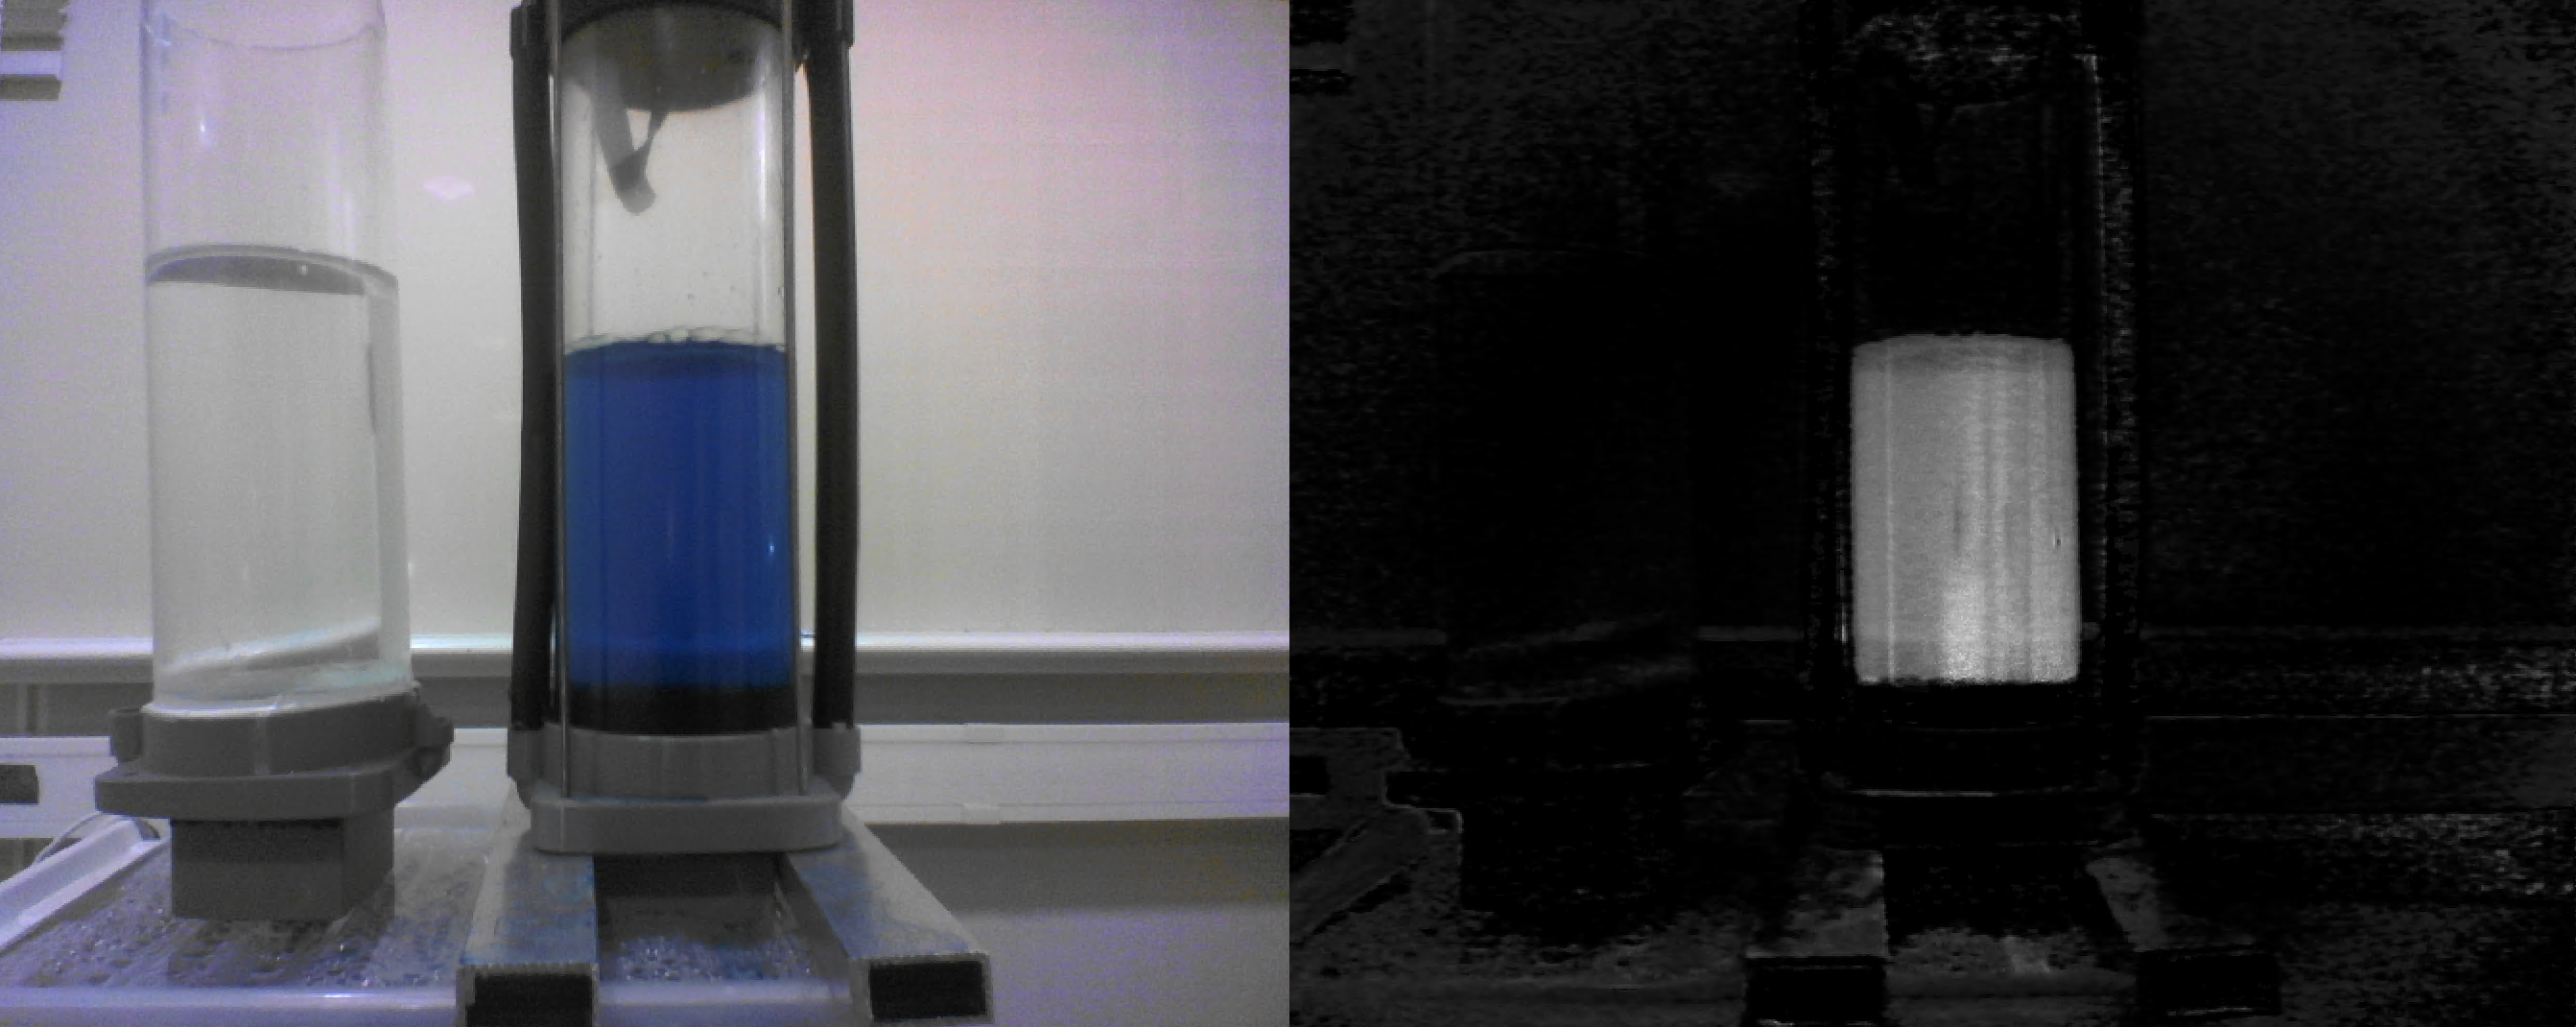
\includegraphics[width=1\textwidth]{pictures/SatRGB}
	\caption{Compearison between raw image (Left) and Saturation plane (Right)}
	\label{img:SRGB}
\end{figure}


As seen in \textbf{Figure \ref{img:SRGB}} The tank containing regular colourless water is almost invisible in the saturation plane while the blue water has become white.

\subsection{Filtering}
By using Fast Fourier Transform \textbf{(FFT)}, the grayscale image is converted into its frequency domain. In the frequency domain of the image, details and sharp edges are recognized as mid to high frequencies. By adding a low pass truncation filter with truncation frequency to 6.00 \%, the unwanted pars of the image becomes filtered out and leaves the blue water alone and easier to detect. The result of the FFT low pass filter are shown in \textbf{Figure \ref{img:FFTS}}.

\begin{comment}
    https://zone.ni.com/reference/en-XX/help/370281M-01/nivisionlvbasics/improve_an_image/ 
\end{comment}

\begin{figure}[b!]
	\centering
	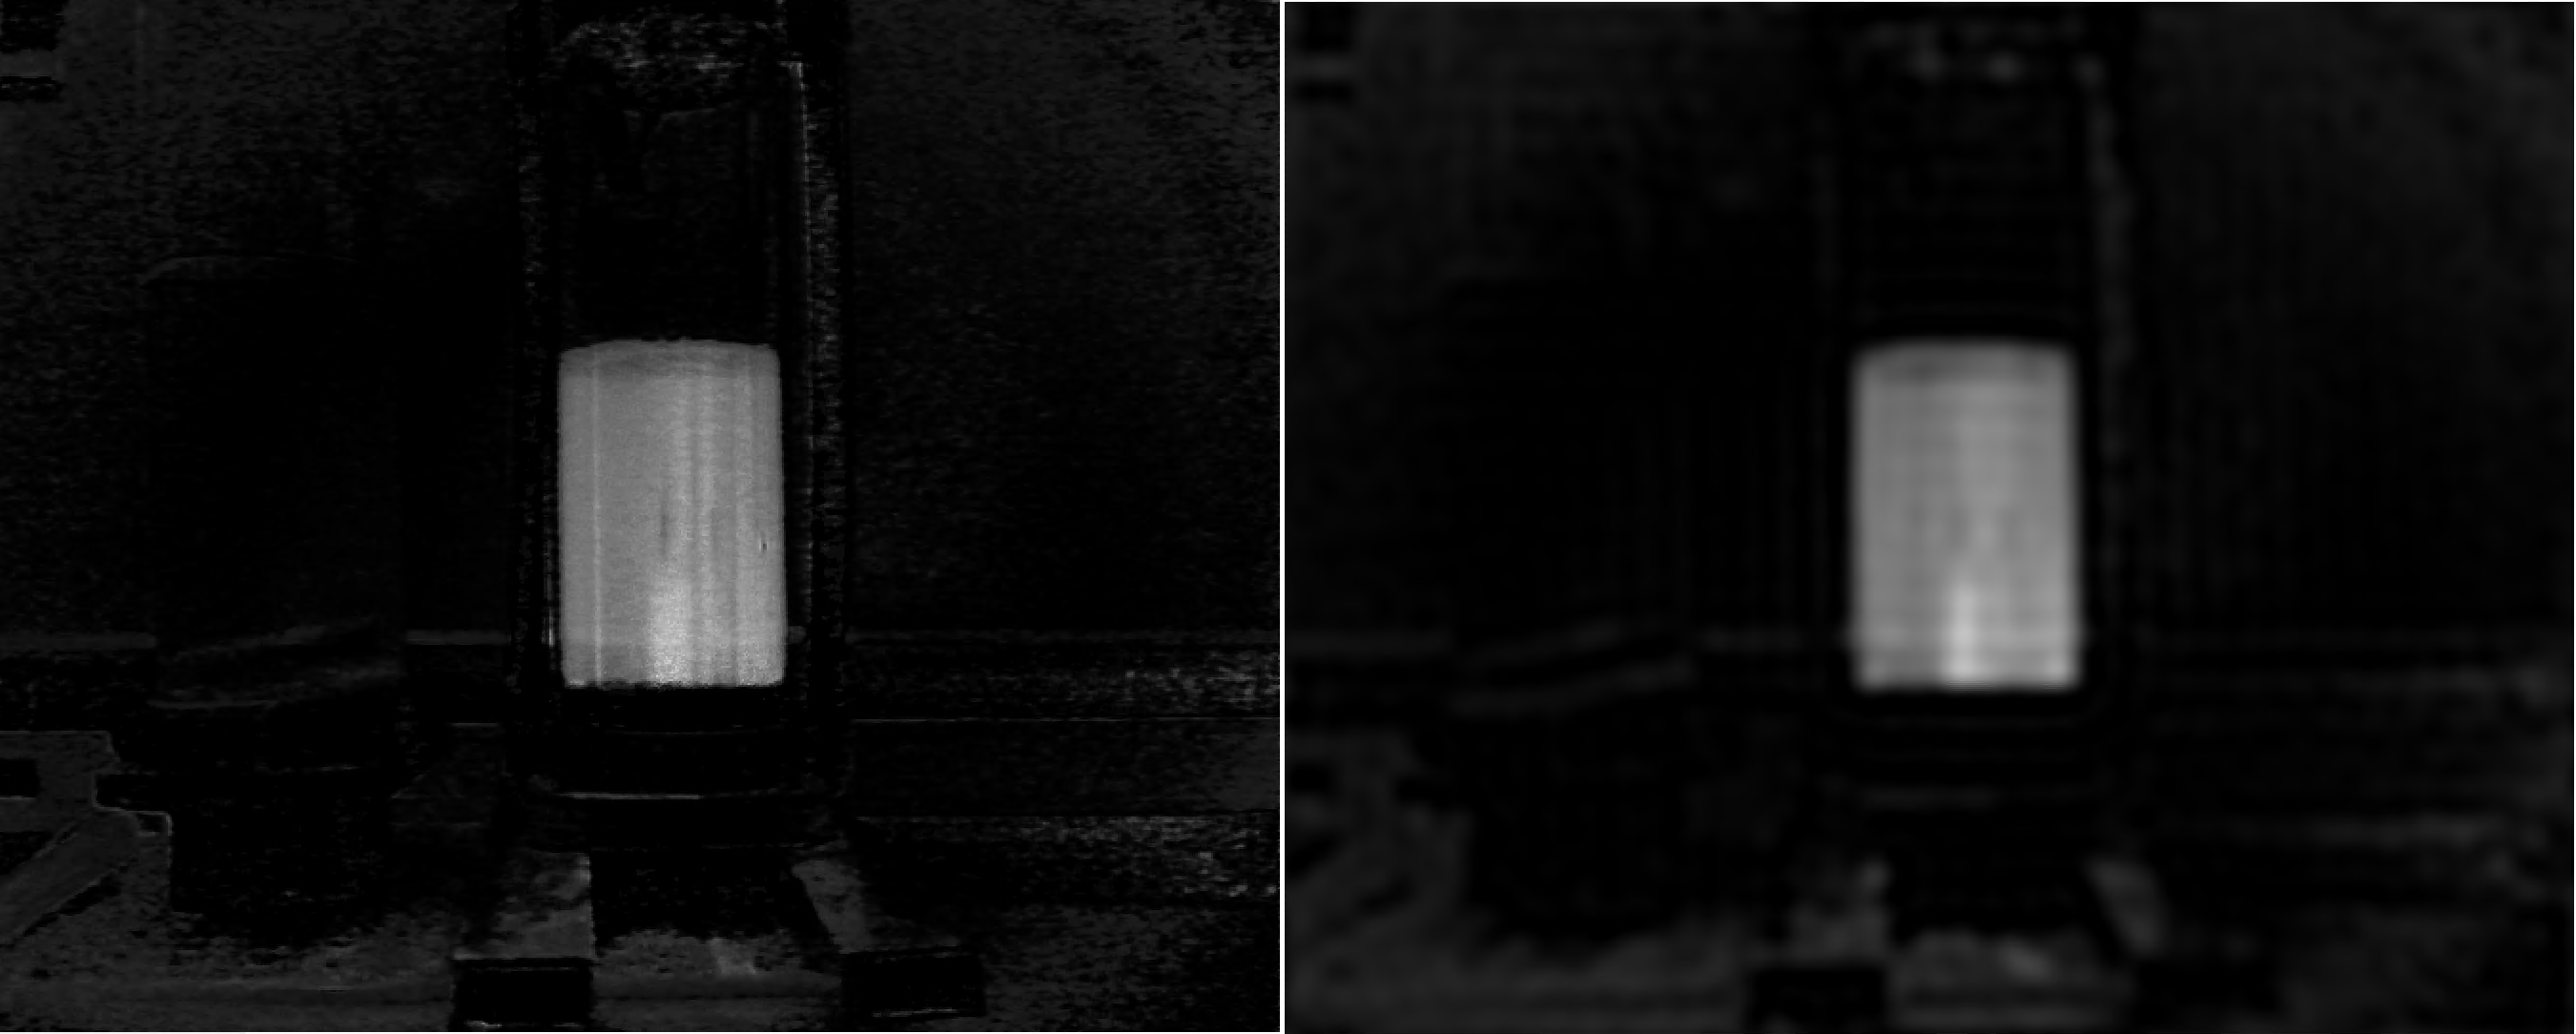
\includegraphics[width=1\textwidth]{pictures/FFTS}
	\caption{Compearison between unfiltered image (Left) and FFT filtered (Right)}
	\label{img:FFTS}
\end{figure}


\subsection{Creating a Binary Image}
The filtered grayscale image starting to become something that is useful to measure the water level with, but there is still some unwanted data in the image. To remove this the image is converted to a binary image by using threshold detection. Since the blue water in the grayscale image is white, the threshold detection was set to look for bright objects. When converting the image to a binary image is the values below 80 in the range 0-255 (0 \% - 100 \%) set to binary 0 and abowe 80 set to binary 1. With this threshold the binary image will be converted to a image with only two values of data in every pixels (\textbf{Figure \ref{img:BIN}}).



\begin{figure}[t!]
	\centering
	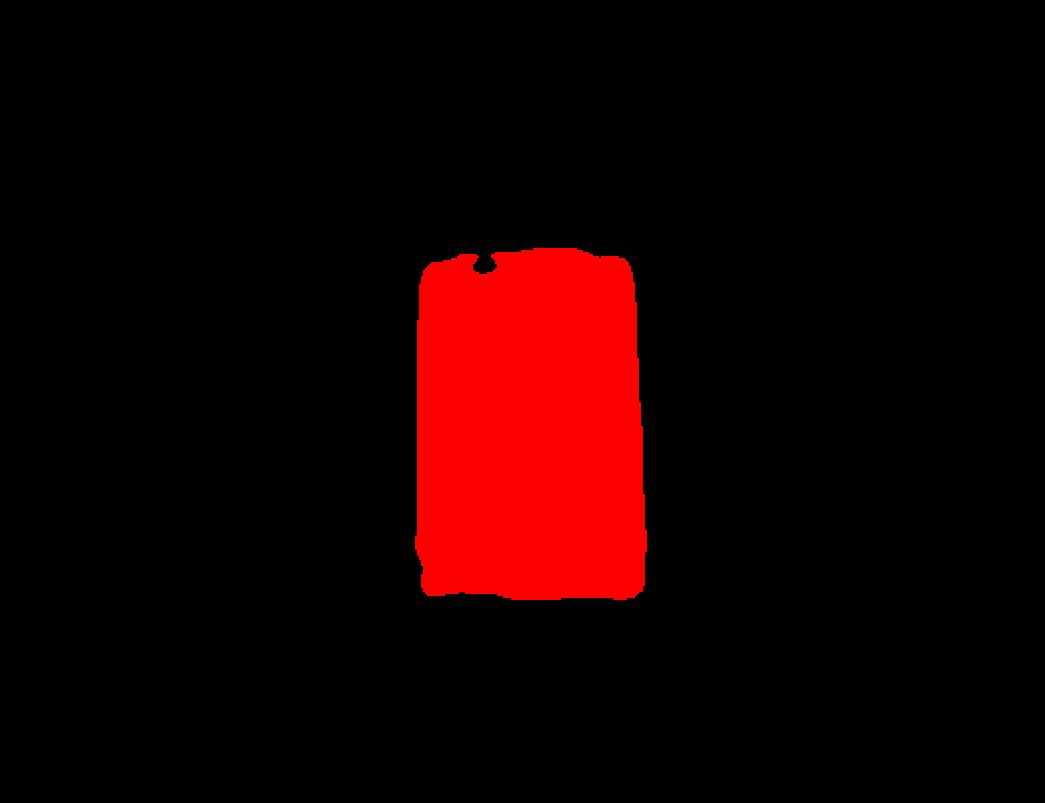
\includegraphics[width=0.75\textwidth]{pictures/BIN}
	\caption{Binary image of the blue water in the drain tank}
	\label{img:BIN}
\end{figure}
%%Dette er kapittel 1 Dette er IMAQ
%%=================================================================
\begin{comment}
\chapter{Image Acquisition} 

\section{Program}

At this state of the project the Glucoset software is not fully automatic. The user have to manually perform a few steps to get a result. In the following chapter contents of the Glucoset software will be described and the steps for an successful measurement of the droplet size will be explained in a step-by-step manual.



\section{Image Acquisition} 

The first part of the Glucoset program is used for the image acquisition from the camera. By using the IMAQdx package from LabVIEW live pictures are imported from the camera into the Glucoset software. The block diagram is shown in Figure \ref{img:Imaq}.

\newpage

\begin{figure}[h!]
	\centering
	\includegraphics[scale=0.35]{ImageAcquisition}
	\caption{LabVIEW block diagram: Image Acquisition}
	\label{img:Imaq}
\end{figure}

It is possible to control different parameters of the camera directly out of the LabVIEW interface. As default, the camera don't give us gray-scaled pictures. Since we choose an algorithm for calculating the drop-volume, in which thresholding is an essential part, we need a grey-scaled image. With the property nodes of the IMAQdx we configure the PixelFormat attribute in the way, that the images are gray-scaled. Furthermore it is possible to modify the ExposureTime attribute of the camera, which can be useful to configure the light environment.
At first the user have only to choose the camera in the LabVIEW interface and click play. Afterwards the live pictures will be displayed in gray-scale in the user interface like shown in Figure \ref{img:pictureGreyscaled}.  

\begin{figure}[h!]
	\centering
	\includegraphics[width=\textwidth]{greyscaled_picture}
	\caption{Greyscaled picture from the camera}
	\label{img:pictureGreyscaled}
\end{figure}

\subsection{Threshold}

With the VI "IMAQ Local Threshold" the gray-scaled picture will be converted into a binary picture in black and white. This binary picture will be needed for the calculation of the droplet volume (See Figure \ref{img:pictureThresholded})


The block diagram is shown in Figure \ref{img:threshold}.

\begin{figure}[h!]
	\centering
	\includegraphics[width=\textwidth]{Thresholding}
	\caption{LabVIEW block diagram: Thresholding}
	\label{img:threshold}
\end{figure} 

By using this VI we can choose different options for the threshold process. 
For this VI the method "Background correction" should be used. This option performs background correction to eliminate non-uniform lighting effects and then performs threshold using the interclass variance threshold algorithm. (LabVIEW Documentation)

We want to find the edge of the cut fiber-cable. The fiber-cable will be gray-scaled while the background will be white because of the light source which is behind the fiber-cable. By using "Look for dark objects" option in the threshold VI the fiber-cable will be displayed in black. 
The "Window size" option is a cluster specifying the size of the window which the VI uses when calculating a local threshold. The best results will be reached with a value of 128x128.


\begin{figure}[h!]
	\centering
	\includegraphics[width=\textwidth]{thresholded_picture}
	\caption{Thresholded picture from the camera}
	\label{img:pictureThresholded}
\end{figure}


\subsection{Edge detection without droplet}

To determine the edges of the fiber-cable (bottom, left, right) we are using the "IMAQ Rake 3" VI. With this VI it is possible to find the left and right edge of the fiber-cable. To determine the bottom, the last pixel of the edges is used. 
In the Figure \ref{img:edgedetection} this VI is in the upper left corner. 

\begin{figure}[h!]
	\centering
	\includegraphics[width=\textwidth]{EdgeDetection}
	\caption{LabVIEW block diagram: Edgedetection}
	\label{img:edgedetection}
\end{figure} 

The ROI Descriptor is used to create a rectangle in which the edges will be searched. Both for-loops are used to find the true left and right edge in case of disturbances in the picture. With this VI we can calculate the width of the fiber-cable and by assuming the width to be 125µm we can calculate the ratio of µm/px.
The calculated width from the picture will be displayed in the user interface. 

\subsubsection{Mask creation}

After the edge detection is completed the mask for the fiber-cable will be created. This mask is a rectangle which will be used to mask the whole area above the bottom of the cut fiber-cable. 
For this we are using the "IMAQ ROIToMask 2" VI. With the edge detection step before we create a ROI Descriptor for the VI with the determined edges. 
Afterwards the mask will be saved as a picture on the disk. The block diagram is shown in Figure \ref{img:MaskCreation}.

\begin{figure}[h!]
	\centering
	\includegraphics[width=\textwidth]{MaskCreation}
	\caption{LabVIEW block diagram: Mask creation}
	\label{img:MaskCreation}
\end{figure} 


\subsubsection{Droplet calculation}

When the mask is created and the droplet afterwards is generated, the droplet calculation can begin. For this we add the mask on the picture of the fiber-cable with the droplet. 
As a result only the droplet is visible because the fibre-cable is masked. (See Figure \ref{img:maskedPicture})

\begin{figure}[h!]
	\centering
	\includegraphics[width=\textwidth]{maskedPicture}
	\caption{Masked threshold from the camera}
	\label{img:maskedPicture}
\end{figure}

In order to calculate the volume of the droplet we are using the "Particle Report" VI. With this VI we can determine all particles in the picture. The block diagram for the particle report is shown in Figure \ref{img:particlereport}.

\begin{figure}[h!]
	\centering
	\includegraphics[width=\textwidth]{ParticleReport}
	\caption{LabVIEW block diagram: Particle Report}
	\label{img:particlereport}
\end{figure} 


By using a for-loop to determine the biggest particle (it is possible that some disturbance pixels are in the picture) we can choose the droplet particle. The detected droplet will be displayed in the User interface. (Like Figure \ref{img:detectedDroplet})

\begin{figure}[h!]
	\centering
	\includegraphics[width=\textwidth]{detectedDroplet}
	\caption{Detected droplet from the Particle Report VI}
	\label{img:detectedDroplet}
\end{figure}

The Dimension of the droplet (in pixels) will be used to calculate the volume of the droplet as its shown in the Figure \ref{img:volumecalculating}. The "width of the fiber cable in pixeln"-attribute at the picture is used to convert the amount of pixel in microns. This attribute was calculated in the edge detection step.   


\begin{figure}[h!]
	\centering
	\includegraphics{CalculatingVolume}
	\caption{LabVIEW block diagram: Volume Calculation}
	\label{img:volumecalculating}
\end{figure} 

The equation we used for the calculations of the volume was:
\begin{equation}
V=\frac{\pi h}{6}\left(3\left(\frac{d}{2}\right)^2+h^2\right) 
\end{equation}
Where V = volume of the droplet, h = height of the droplet from the fiber to the tip of the droplet and d = diameter or width of the droplet.

\newpage
\subsubsection{Overview}

At Figure \ref{img:OverviewCompleteProgram} you can see the whole LabVIEW block diagram.

\begin{figure}[h!]
	\centering
	\includegraphics[width=\textwidth]{OverviewCompleteProgram}
	\caption{Overview of the block diagram}
	\label{img:OverviewCompleteProgram}
\end{figure} 

	
\end{comment}

%
% Må gjerne flyttes/endres på osv
% Samle et kapittel for testplatformen? Med soft- og hardware?
%
\begin{comment} 
\chapter{Test Platform}


\section{Control Software}

To be able to automate a sequence of measurements a control GUI was created in LabVIEW.


\subsection{Motor Controls}

There are two options available to control the motors from LabVIEW. One low-level method by sending binary commands directly to the motor serial port, this requires manually constructed command packages and a robust read and write system for transmission.
Another method is using a third-party ActiveX component which runs in the background (\cref{fig:thorlabsAPT}), this software is provided for free by Thorlabs. This solution enables the use of ActiveX properties within LabVIEW and was therefore chosen.
%, and since a cross-platform end product was not a requirement this solution was chosen.

\begin{figure}
	\centering
	\includegraphics[width=0.8\textwidth]{Thorlabs_APT_config}
	\caption{Thorlabs APT software in simulator mode.}
	\label{fig:thorlabsAPT}
\end{figure}


The ActiveX component contributed to some stability issues regarding the connection to the motors, and it also makes this control software platform dependent. But it has a built in simulator and preset command properties which makes development and debugging a lot easier.


\subsection{Control Interface}

When the control interface initiates a configuration window as shown in \cref{fig:confguiv1} will be visible. The configuration requires the motor serial numbers for all three axis, the serial port source for the light control and the camera port source. The latter two is optional in current version.

\begin{figure}
	\centering
	\includegraphics[width=0.5\textwidth]{GlucosetGUI_conf_v1}
	\caption{Configuration GUI}
	\label{fig:confguiv1}
\end{figure}

Each serial number input has an indicator next to it that turns light green (on) when the motor is connected correctly. When all three motors are connected the main control window as shown in \cref{fig:mainguiv1} is made available. 

\begin{figure}
	\centering
	\includegraphics[width=\textwidth]{GlucosetGUI_main_v1}
	\caption{Main control GUI}
	\label{fig:mainguiv1}
\end{figure}

The left side in the main window contains the manual motor controls. Where it is possible to set the maximum motor velocity, acceleration and position of the Z-axis (axis that holds the fiber optics).

A jogging panel is provided to easily control all three axis of the test platform. The ``Go Home'' function will send the linear stages to their home position, default is $0.000$ which is the beginning of the stage. And the ``Set Home'' function is supposed to set current position as home, but this functionality is not yet implemented.


\subsection{Test Run Configuration}

The right side of the main window contains the test procedure settings.

``Start Position'' (\cref{fig:testprocstart}) is the Z-axis position before and after a completed test run. This position is added for maintenance of the fiber optic when a test sequence is complete.

``Camera Position'' (\cref{fig:testproccam}), where the image acquisition is being done, and ``Stop Position'' (\cref{fig:testprocstop}) is the positions the test will switch between in a test run.

The test run behavior is configured by setting the start velocity, velocity increment and stop velocity where the test run is considered complete. A delay at the stop position can also be added if necessary.

\begin{figure}[h]
    \centering
    \begin{subfigure}{0.33\textwidth}
        \centering
        \includegraphics[width=0.5\linewidth]{start_pos}
        \caption{Start Position}
        \label{fig:testprocstart}
    \end{subfigure}%
    \begin{subfigure}{0.33\textwidth}
        \centering
        \includegraphics[width=0.5\linewidth]{cam_pos}
        \caption{Camera Position}
        \label{fig:testproccam}
    \end{subfigure}%
    \begin{subfigure}{0.33\textwidth}
        \centering
        \includegraphics[width=0.5\linewidth]{stop_pos}
        \caption{Stop Position}
        \label{fig:testprocstop}
    \end{subfigure}
    \caption{Test sequence positions}
    \label{fig:testprocstages}
\end{figure}



\subsection{Current Status}

While this first version of the control software works, both manual motor control and the test procedure as described above, it has not been tested in combination with the IMAQ system. The fiber optic requires a manual cleansing between each take, and this user controlled pause has not been implemented.

A more complete version of the interface, as shown in \cref{fig:mainguiv2}, was in development. But due to time constrains of this project and difficulties with the automation of the IMAQ-system the development was halted. 


\begin{figure}[h!]
    \centering
	\includegraphics[width=0.9\textwidth]{GlucosetGUI_main_v2}
	\caption{Main control GUI, second version}
	\label{fig:mainguiv2}
\end{figure}
\end{comment}
\begin{comment}
\chapter{Testing and results}

All of the droplet volume tests has been performed according to the step by step manual for the user, wich can be found in appendix \ref{cha:Test procedure}. This chapter will present additional elements in the test procedure, present the test results and discuss them. 

Originally the fiber should be immersed in a beacer of two liquid solutions: Squalane oil and distilled water. Squalane oil is lighter than distilled water, and we would therefore measure the size of the water droplet when it came from the distilled water into squalane oil.
Measuring the size of a droplet through the beacer proved to be a difficult task, partly because of the refractive index in the beacer and the distribution of light. 
It was therefore tried to measure the droplet size of distilled water into the air, but since the drop has time to evaporate before a picture is taken, this is not feasible at this time. It was therefore decided that we measure the droplet size of squalane oil in air,since this oil doesn't evaporate at the same rate as distilled water. It is not the best solution in relation to use in real life, but is currently the best solution to carry out final measurements.


The tests have been performed with four acceleration values: 0.5 , 1.0 , 1.5 and 2.0   $mm/s^2$

The tests have been conducted in three separate series, where the goal was to see if there is any correlation of speed and droplet volume.

The same start and stop position has been used for all attempts in each serie, but the three series have different start- and stop positions, resulting in varying travel length for the fiber. 
Travel length serie 1: 1,3 mm
Travel length serie 2: 2,0 mm
Travel length serie 3: 2,0 mm


\section{Test results}
Complete test results from test series 1-3 can be found in Appendix \ref{cha:test_res}. On the next page one can see graphical displays of the results from the test series. 



\begin{figure}[h!]
	\centering
	\includegraphics[scale=0.65]{pictures/FinVolTest/Combined/Acc0_5L}
	\caption{Three test series. Acceleration: $0.5$ $mm/s^2$}
	\label{img:Acc0_5}
\end{figure}

\begin{figure}[h!]
	\centering
	\includegraphics[scale=0.65]{pictures/FinVolTest/Combined/Acc1_0L}
	\caption{Three test series. Acceleration: $1.0$ $mm/s^2$}
	\label{img:Acc1_0}
\end{figure}

\begin{figure}[h!]
	\centering
	\includegraphics[scale=0.65]{pictures/FinVolTest/Combined/Acc1_5L}
	\caption{Three test series. Acceleration: $1.5$ $mm/s^2$}
	\label{img:Acc1_5}
\end{figure}

\begin{figure}[h!]
	\centering
	\includegraphics[scale=0.65]{pictures/FinVolTest/Combined/Acc2_0L}
	\caption{Three test series. Acceleration: $2.0$ $mm/s^2$}
	\label{img:Acc2_0}
\end{figure}


\newpage

\section{Comments}
Figure \ref{img:Acc0_5} to \ref{img:Acc2_0} shows that there is no correlation in the test results between the three series.



During the test procedure we experienced that the measured volume changed more than expected, and that the two measurements that would give the same results were not near each other. The width of a droplet could be measured to be approximately 4000 um, a size that is clearly not possible to achieve. Those results are considered corrupted and are thus neglected.

The volume of the droplet was also calculated with a fixed width of 125 um for some of the datasets, but with no good result. The data points in the curve is more evenly distributed, but the curve still doesnt have the desired curvature.

\begin{figure}[!ht]
	\centering
	\includegraphics[width=0.7\textwidth]{pictures/FinVolTest/Vol_m_vs_f_width}
	\caption{Comparison: Calculated droplet volume with measured width and fixed width}
	\label{img:m_vs_f}
\end{figure}

\end{comment}
\begin{comment}

\addcontentsline{toc}{section}{Conclusion}
\chapter{Conclusion}
 the relationship between travel length, speed and droplet formation 
The mechanical setup using Thorlabs works satisfactory. The merge between Thorlabs hardware and other hardware has also been implemented with success. There are however some hardware-related issues that affects the measurements, and limits the possibilities for complete testing and software development. 

A software for measurements of volume in a droplet has been created, and it produces results that to some extent gives plausible results. We do however not have the knowledge or equipment to cross check these results and perform volume measurements of a droplet to compare with our results. As mentioned in the chapter Testing and Results the droplet width was sometimes measured to be significantly larger than the actual size. Since the width of the fiber cable is fixed with a width of 125 $\mu$ m the droplet width can not have a width higher than this. If we set the width of the fiber cable fixed at 125 $\mu$ m, the process of masking this area is simplified, but it doesn't explain the large variances seen in the droplet volume as it is only one factor in the measurements. 

In order to produce results that are scientifically more accurate one would have to do changes to both hardware and software. The camera we used for our measurements does not have auto focus. This means that for each sample the camera has to be manually focused. This has been done by moving the camera on the x- and y-axis. This process changes the distance between the camera and the fiber cable, and the uncertainty of volume measurements are greatly increased as a consequence. Obtaining a camera with auto focus would greatly increase the chances of being able to reproduce results. 

Provided the changes to the mechanical setup is implemented, an automatized test routine could be implemented. The test platform described in chapter 3 could be used for this purpose. In this scenario a mask would not be needed in between each sample measurement, this would give a higher accuracy of measurements. This would also enable extensive series testing. This would give a better indicator of the accuracy of the system, and a better basis for research on the relationship between travel length, speed and droplet formation.  

The masking of the droplet is essential in producing an accurate measurement of volume. The current method should be enhanced. 

\end{comment}



\begin{appendices}


\begin{comment}
\chapter{Step by Step manual for the user} \label{cha:Test procedure}

\section{Step by Step manual for the user} 

\begin{figure}[h!]
	\centering
	\includegraphics[scale=0.4]{UserInterface}
	\caption{User Interface}
	\label{img:UserInterface}
\end{figure} 

\newpage
\renewcommand{\labelenumi}{\Roman{enumi}.}
\begin{enumerate}
\item Select the camera name in the User interface which should be used for the droplet detection. 
\item Select the COM-port which is used for the light control.
\item Run the VI.
\item Drive the fiber-cable in a fix exact position in the scope of the camera by using Thorlabs APT User. Remember the position.
\item Adjust the focus for sharp edges. 
\item Choose the threshold options:

\begin{itemize}
\item Look for: Dark options
\item Method: Background
\item Window Size: 128x128
\end{itemize}
							
\item Press "Detect without droplet". (This will save the picture on your disk and the mask will be created)
\item Drive the fiber-cable down to create a droplet and drive it back exactly in the remembered position. 
\item Press "Detect with droplet" (This picture will be saved)
\item Press "Use Mask"
\item Press "Find particles" (Calculation of the volume) 
\end{enumerate}
\end{comment}

% Table generated by Excel2LaTeX from sheet 'Ark 1'
\chapter{Test results} \label{cha:test_res}

\begin{table}[htbp]
  \centering
  \caption{Test results - Series \# 1  }
  %Travel length: 1.3 mm  How do I add this as a line under the table-text?
    \begin{tabular}{rrrrr}
    \toprule
    Acceleration & Velocity & Volume [\textmu m$^3$]  & Height [\textmu m] & Width [\textmu m] \\
    \midrule
    0,5   & 0,5   & 249541 & 38,1737 & 121,257 \\
    0,5   & 0,6   & 249808 & 38,3266 & 120,002 \\
    0,5   & 0,8   & 223667 & 35,489 & 119,874 \\
    0,5   & 1     & 252836 & 38,4809 & 121,479 \\
    0,5   & 1,2   & 200369 & 34,7432 & 117,825 \\
    0,5   & 1,4   & 255900 & 38,1874 & 122,963 \\
    0,5   & 1,6   & 226512 & 35,6061 & 120,455 \\
    0,5   & 1,8   & 223968 & 35,6061 & 119,697 \\
    0,5   & 2     & 240961 & 37,1212 & 121,212 \\
          &       &       &       &  \\
    1     & 0,6   & 227008 & 36,2173 & 119,215 \\
    1     & 0,8   & 255433 & 38,7538 & 121,581 \\
    1     & 1     & 232607 & 36,8236 & 119,489 \\
    1     & 1,2   & 248509 & 37,9555 & 121,458 \\
    1     & 1,4   & 254644 & 38,2653 & 122,449 \\
    1     & 1,6   & 244773 & 37,7643 & 120,846 \\
    1     & 1,8   & 210097 & 34,6734 & 117,588 \\
    1     & 2     & 225991 & 36,4372 & 118,421 \\
          &       &       &       &  \\
    1,5   & 0,6   & 203996 & 33,8855 & 117,47 \\
    1,5   & 0,8   & 211369 & 34,7432 & 117,825 \\
    1,5   & 1     & 267442 & 39,5132 & 123,1 \\
    1,5   & 1,2   & 196885 & 33,1658 & 116,834 \\
    1,5   & 1,4   & 229771 & 36,3636 & 119,697 \\
    1,5   & 1,6   & 202439 & 34,1945 & 116,261 \\
    1,5   & 1,8   & 233511 & 37,0091 & 119,335 \\
    1,5   & 2     & 186037 & 33,4074 & 114,969 \\
          &       &       &       &  \\
    2     & 0,6   & 229771 & 36,3636 & 119,697 \\
    2     & 0,8   & 220930 & 35,7143 & 118,541 \\
    2     & 1     & 187682 & 32,4447 & 115,443 \\
    2     & 1,2   & 265101 & 38,9511 & 123,727 \\
    2     & 1,4   & 251316 & 38,4036 & 121,235 \\
    2     & 1,6   & 261832 & 39,2354 & 122,233 \\
    2     & 1,8   & 264073 & 39,6341 & 121,951 \\
    2     & 2     & 199317 & 33,8855 & 115,964 \\
    \bottomrule
    \end{tabular}%
  \label{tab:test1}%
\end{table}%

% Table generated by Excel2LaTeX from sheet 'Ark 1'


\begin{table}[htbp]
  \centering
  \caption{Test results - Series \# 2}
  %Travel length: 2.0 mm  How do I add this as a line under the table-text?
    \begin{tabular}{rrrrr}
    \toprule
    Acceleration & Velocity & Volume [\textmu m$^3$] & Height [\textmu m] & Width [\textmu m] \\
    \midrule
    0,5   &       &       &       &  \\
    0,5   & 0,6   & 255897 & 30,0782 & 120,992 \\
    0,5   & 0,8   & 315966 & 45,7019 & 128,106 \\
    0,5   & 1     & 564854 & 65,184 & 128,067 \\
    0,5   & 1,2   & 236642 & 36,2654 & 121,914 \\
    0,5   & 1,4   & 198849 & 32,6087 & 118,789 \\
    0,5   & 1,6   & 287837 & 41,25 & 124,5 \\
    0,5   & 1,8   & 292974 & 40,8951 & 126,543 \\
    0,5   & 2     & 276227 & 40,5405 & 123,123 \\
          &       &       &       &  \\
    1     & 0,6   & 275345 & 39,7554 & 124,618 \\
    1     & 0,8   & 296681 & 42,2535 & 124,497 \\
    1     & 1     & 340355 & 44,5312 & 129,687 \\
    1     & 1,2   & 289486 & 41,0334 & 125,38 \\
    1     & 1,4   & 254078 & 38,4036 & 121,988 \\
    1     & 1,6   & 291253 & 41,1168 & 125,635 \\
    1     & 1,8   & 217222 & 35,061 & 118,902 \\
    1     & 2     & 277877 & 39,8773 & 125 \\
          &       &       &       &  \\
    1,5   & 0,6   & 269046 & 39,75 & 123 \\
    1,5   & 0,8   & 268367 & 39,1104 & 124,233 \\
    1,5   & 1     & 260258 & 39,1566 & 121,988 \\
    1,5   & 1,2   & 276587 & 39,959 & 124,488 \\
    1,5   & 1,4   & 271482 & 39,8696 & 123,37 \\
    1,5   & 1,6   & 306887 & 42,4383 & 126,543 \\
    1,5   & 1,8   & 251777 & 37,8086 & 122,685 \\
    1,5   & 2     & 284821 & 41,25 & 123,75 \\
          &       &       &       &  \\
    2     & 0,6   & 288267 & 41,4157 & 124,247 \\
    2     & 0,8   & 278342 & 40,5  & 123,75 \\
    2     & 1     & 228090 & 35,8232 & 120,427 \\
    2     & 1,2   & 211879 & 34,6386 & 118,223 \\
    2     & 1,4   & 269855 & 39,7898 & 123,123 \\
    2     & 1,6   & 228195 & 36,1446 & 119,729 \\
    2     & 1,8   & 275345 & 39,7554 & 124,618 \\
    2     & 2     & 276227 & 40,5405 & 123,123 \\
    \bottomrule
    \end{tabular}%
  \label{tab:test2}%
\end{table}%

% Table generated by Excel2LaTeX from sheet 'Ark 1'


\begin{table}[htbp]
  \centering
  \caption{Test results - Series \# 3}
  %Travel length: 2.0 mm  How do I add this as a line under the table-text?
    \begin{tabular}{rrrrr}
    \toprule
    Acceleration & Velocity & Volume [\textmu m$^3$] & Height [\textmu m] & Width [\textmu m] \\
    \midrule
    0,5   &       &       &       &  \\
    0,5   & 0,6   & 247793 & 37,9464 & 121,28 \\
    0,5   & 0,8   & 284411 & 41,0857 & 124,004 \\
    0,5   & 1     & 250122 & 37,2671 & 123,447 \\
    0,5   & 1,2   & 273368 & 39,3519 & 125 \\
    0,5   & 1,4   & 265450 & 39,1104 & 123,466 \\
    0,5   & 1,6   & 270020 & 39,1906 & 124,488 \\
    0,5   & 1,8   & 234494 & 36,4742 & 120,821 \\
    0,5   & 2     & 288702 & 41,2913 & 124,625 \\
          &       &       &       &  \\
    1     & 0,6   & 273368 & 39,3519 & 125 \\
    1     & 0,8   & 296585 & 40,7523 & 127,743 \\
    1     & 1     & 306610 & 43,0081 & 125,252 \\
    1     & 1,2   & 242328 & 37,5  & 120,75 \\
    1     & 1,4   & 281325 & 40,0411 & 125,513 \\
    1     & 1,6   & 238333 & 36,8098 & 121,166 \\
    1     & 1,8   & 286862 & 40,9091 & 125 \\
    1     & 2     & 287837 & 41,25 & 124,5 \\
          &       &       &       &  \\
    1,5   & 0,6   & 284545 & 40,6442 & 125 \\
    1,5   & 0,8   & 307881 & 43,5  & 124,5 \\
    1,5   & 1     & 303096 & 41,6667 & 127,315 \\
    1,5   & 1,2   & 287400 & 41,3741 & 124,122 \\
    1,5   & 1,4   & 242328 & 37,5  & 120,75 \\
    1,5   & 1,6   & 247172 & 37,5767 & 121,933 \\
    1,5   & 1,8   & 287400 & 41,3741 & 124,122 \\
    1,5   & 2     & 341281 & 45,6186 & 127,577 \\
          &       &       &       &  \\
    2     & 0,6   & 278493 & 39,5963 & 125,776 \\
    2     & 0,8   & 248313 & 38,25 & 120,75 \\
    2     & 1     & 268367 & 39,1104 & 124,233 \\
    2     & 1,2   & 289053 & 41,1585 & 125 \\
    2     & 1,4   & 283829 & 40,9091 & 124,242 \\
    2     & 1,6   & 276679 & 40,4192 & 123,503 \\
    2     & 1,8   & 261043 & 39,196 & 122,111 \\
    2     & 2     & 283119 & 41,1677 & 123,503 \\
    \bottomrule
    \end{tabular}%
  \label{tab:test3}%
\end{table}%

    
\chapter{Equipment hardware platform} \label{cha:equipment}



These are the main components of the Thorlabs hardware setup:
\begin{compactitem}
\item Thorlabs Z825B DC Servo motor
\item Thorlabs TDC001 DC Servo motor Controller
\item Thorlabs PT 102 right angle bracket
\item Thorlabs PT1 Single axis translation stage
\item Thorlabs Ø1/2" Post Holders, angle clamps and other related accesories
\item Thorlabs T711-250 Fiber clamp
\item Thorlabs MB12 Solid aluminium optical breadboard
\end{compactitem}


\begin{comment}
\chapter{LED driver shield schematics} \label{cha:ERM_APX2}

\vfill

\begin{figure}[h!]
	\centering
	\includegraphics[height=1\textheight]{pictures/LabLight_Schematics}
\end{figure}
\clearpage
\end{comment}
\chapter{Controller board firmware} \label{cha:ERM_APX1}


\lstset{language=C++,
        basicstyle=\scriptsize\ttfamily,
        keywordstyle=\scriptsize\color{blue}\ttfamily,
        stringstyle=\scriptsize\color{red}\ttfamily,
        commentstyle=\scriptsize\color{black}\ttfamily,
        morecomment=\scriptsize[l][\color{magenta}]{\#}
}

\section{Main function} \label{cha:ERM_APX1_1}

\begin{lstlisting}

#include <stdio.h>
#include <avr/io.h>
#include <avr/interrupt.h>

#define F_CPU 11059200UL    // External 11,0592 MHz oscillator fuse activated
#include <util/delay.h>

int main(void){
    uart_init(F_CPU,57600);     // Initialize UART communication, 57600 baud
    pwm_init();                 // Initialize PWM
    set_bright(0);              // Turn off LEDs
    sei();                      // Enable global interrupts
    
    while(1){
        // Do nothing
    }
}

ISR(USART1_RX_vect){    // Interrupt routine triggered by received USART communication
    char temp;
    temp = UDR1;        // Store received character
    set_bright(temp);   // Set new duty cycle
    UDR1 = temp;        // Echo back received character
}

\end{lstlisting}
\clearpage


\section{UART initialization and send function} \label{cha:ERM_APX1_2}

\begin{lstlisting}[language=C++]

#include <avr/io.h>	

void uart_init(uint32_t f_cpu,uint32_t baud);
void uart_send(char *str);

void uart_init(uint32_t f_cpu, uint32_t baud){
    uint16_t baud_rate = ((f_cpu/(16*baud))-1);
    UCSR1B |= ((1<<RXEN1)|(1<<TXEN1));          // Enable UART receiver and transmitter
    UBRR1H |= baud_rate >> 8;                   // Set baud rate high byte
    UBRR1L |= baud_rate;                        // Set baud rate low byte
    UCSR1B |= (1<<RXCIE1);                      // Enable receiver interrupt
}

void uart_send(char *str){
    while (*str){
        while (!(UCSR1A & (1<<UDRE1))){
            // Wait for transmission to end
        }
        UDR1 = *str;        // Transmit character
        str++;              // Advance string position
    }
}

\end{lstlisting}
\clearpage


\section{PWM initialization and set brightness function} \label{cha:ERM_APX1_3}

\begin{lstlisting}[language=C++]

#include <avr/io.h>

void pwm_init(void);
void set_bright(uint8_t bright);

void pwm_init(void){
    DDRB |= (1<<PORTB3);                    // Set LED1 (PB3) as output
    TCCR0A |= ((1<<WGM01)|(1<<WGM00));      // Initialize fast PWM mode
    TCCR0A |= (1<<COM0A1);                  // Clear PB3 on compare match, 
                                            // set on BOTTOM (non-inverting mode)
    TCCR0B |= ((1<<CS01)|(1<<CS00));        // Set 1/64 prescaler
}

void set_bright(uint8_t bright){
    if (bright == 0){
        TCCR0A = 0;                         // Disable PWM
    }
    else{
        pwm_init();                         // Reenable PWM
        OCR0A = bright;                     // Set counter to clear on bright
    }
}

\end{lstlisting}
\clearpage



\end{appendices}



\end{document}

